\documentclass[12pt,a4paper]{article}
\usepackage[utf8]{inputenc}
\usepackage[margin=1in]{geometry}
\usepackage{graphicx}
\usepackage{listings}
\usepackage{xcolor}
\usepackage{amsmath}
\usepackage{fancyhdr}
\usepackage{titlesec}
\usepackage{hyperref}
\usepackage{float}

% Code listing style
\definecolor{codegreen}{rgb}{0,0.6,0}
\definecolor{codegray}{rgb}{0.5,0.5,0.5}
\definecolor{codepurple}{rgb}{0.58,0,0.82}
\definecolor{backcolour}{rgb}{0.95,0.95,0.92}

\lstdefinestyle{mystyle}{
    backgroundcolor=\color{backcolour},   
    commentstyle=\color{codegreen},
    keywordstyle=\color{magenta},
    numberstyle=\tiny\color{codegray},
    stringstyle=\color{codepurple},
    basicstyle=\ttfamily\footnotesize,
    breakatwhitespace=false,         
    breaklines=true,                 
    captionpos=b,                    
    keepspaces=true,                 
    numbers=left,                    
    numbersep=5pt,                  
    showspaces=false,                
    showstringspaces=false,
    showtabs=false,                  
    tabsize=4
}
\lstset{style=mystyle}

% Header and Footer
\pagestyle{fancy}
\fancyhf{}
\rhead{Computer Graphics Lab}
\lhead{Lab 3}
\rfoot{Page \thepage}

\begin{document}

% Title Page
\begin{titlepage}
    \centering
    \vspace*{1cm}
    
    \Huge
    \textbf{Computer Graphics Laboratory}
    
    \vspace{0.5cm}
    \LARGE
    Lab Report 3
    
    \vspace{1.5cm}
    
    \Large
    \textbf{2D Transformations using Homogeneous Coordinates}
    
    \vspace{2cm}
    
    \textbf{Submitted By:}\\
    \vspace{0.3cm}
    \Large
    Student Name
    
    \vspace{2cm}
    
    \textbf{Date:}\\
    \vspace{0.3cm}
    \today
    
    \vfill
    
    \large
    Department of Computer Science\\
    5th Semester
    
\end{titlepage}

\tableofcontents
\newpage

%===========================================
% TASK 1: 2D TRANSLATION
%===========================================
\section{2D Translation}

\subsection{Title of Lab Activity}
Implementation of 2D Translation transformation using homogeneous coordinate system to move objects from one position to another.

\subsection{Algorithm used for drawing line}
Digital Differential Analyzer (DDA) and Bresenham's line algorithm are commonly used for rasterizing lines. For visualization purposes, we use Matplotlib's vector plotting which handles line rendering internally.

\textbf{Translation Algorithm Steps:}
\begin{enumerate}
    \item Input the translation distances: $t_x$ (horizontal) and $t_y$ (vertical)
    \item Construct the translation matrix:
    $$T = \begin{bmatrix} 1 & 0 & t_x \\ 0 & 1 & t_y \\ 0 & 0 & 1 \end{bmatrix}$$
    \item Convert 2D points $(x, y)$ to homogeneous coordinates $(x, y, 1)$
    \item Apply transformation: $P' = T \times P$
    \item Extract translated coordinates from result
\end{enumerate}

\subsection{Source Code}
\begin{lstlisting}[language=Python, caption=2D Translation Implementation]
@staticmethod
def translation_matrix(tx, ty):
    """
    Create a translation transformation matrix.
    
    Args:
        tx: Translation in x-axis
        ty: Translation in y-axis
        
    Returns:
        3x3 translation matrix
    """
    return np.array([
        [1, 0, tx],
        [0, 1, ty],
        [0, 0, 1]
    ], dtype=float)

# Example usage
rect = Shape2D([(0, 0), (3, 0), (3, 2), (0, 2)], name="Rectangle")
trans = Transformation2D.translation_matrix(5, 2)
rect.apply_transformation(trans)
Visualizer2D.plot_comparison(original_rect, rect, title="2D Translation")
\end{lstlisting}

\subsection{Output}
\begin{figure}[H]
    \centering
    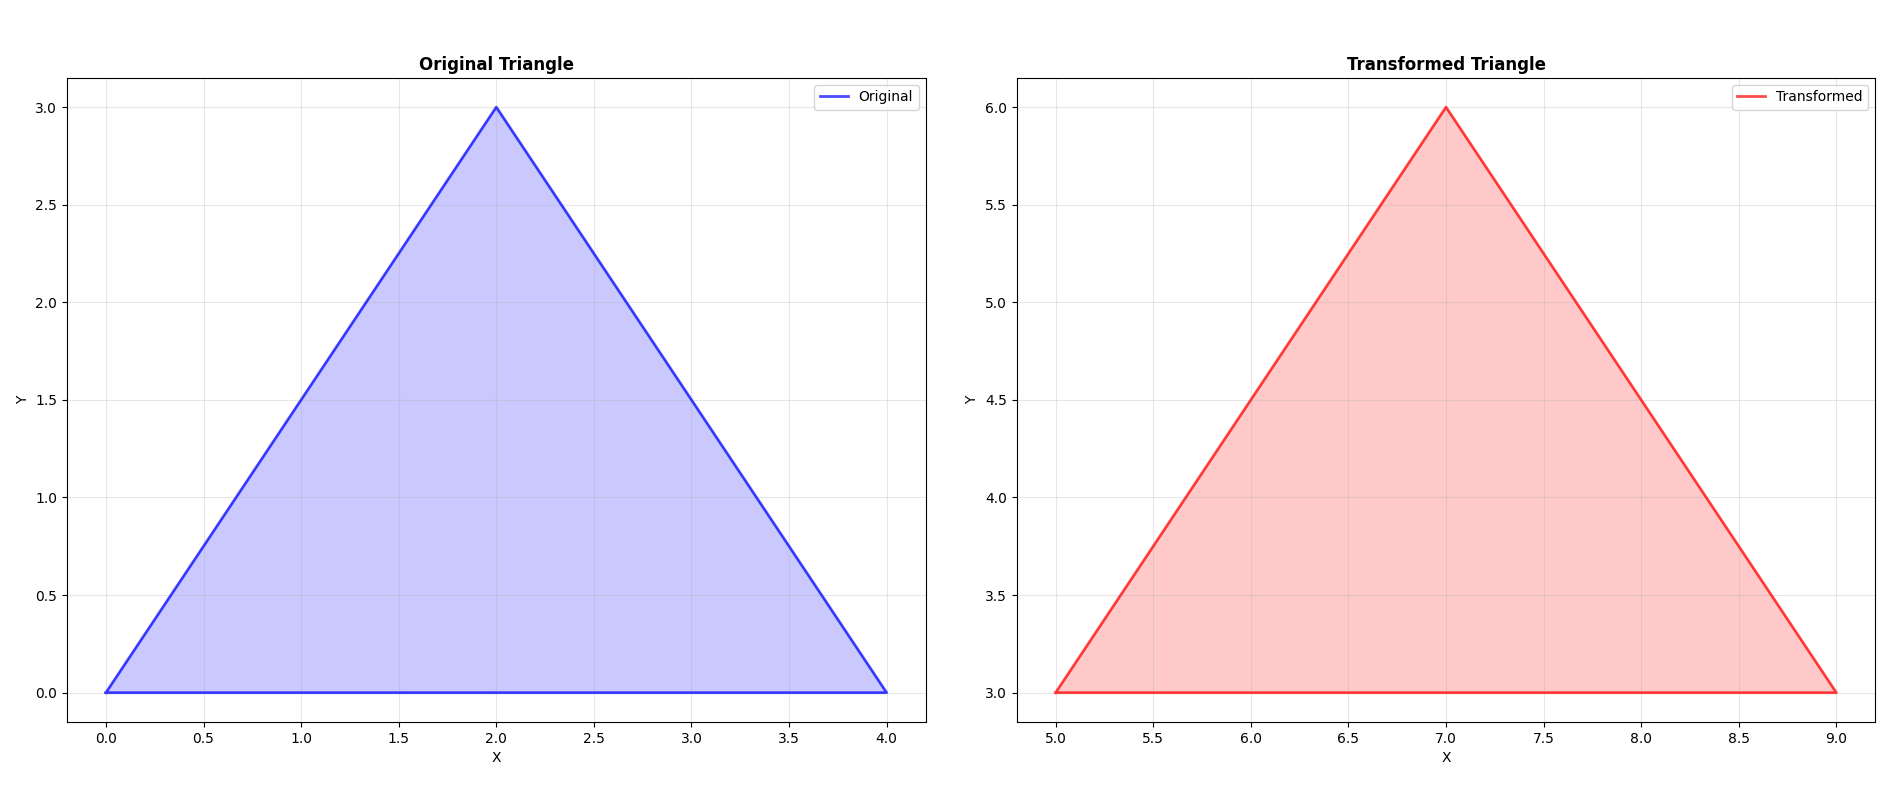
\includegraphics[width=0.8\textwidth]{fig/Screenshot 2026-02-09 154048.png}
    \caption{2D Translation: Original shape (left) vs Translated shape (right)}
\end{figure}

\newpage
%===========================================
% TASK 2: 2D ROTATION
%===========================================
\section{2D Rotation}

\subsection{Title of Lab Activity}
Implementation of 2D Rotation transformation using homogeneous coordinates to rotate objects about the origin by a specified angle.

\subsection{Algorithm used for drawing line}
Digital Differential Analyzer (DDA) and Bresenham's line algorithm are standard methods for line rasterization. The visualization employs Matplotlib's plotting capabilities for smooth rendering.

\textbf{Rotation Algorithm Steps:}
\begin{enumerate}
    \item Input the rotation angle $\theta$ (in degrees)
    \item Convert angle to radians: $\theta_{rad} = \theta \times \frac{\pi}{180}$
    \item Construct the rotation matrix:
    $$R = \begin{bmatrix} \cos\theta & -\sin\theta & 0 \\ \sin\theta & \cos\theta & 0 \\ 0 & 0 & 1 \end{bmatrix}$$
    \item Convert 2D points to homogeneous coordinates
    \item Apply transformation: $P' = R \times P$
    \item Extract rotated coordinates from result
\end{enumerate}

\subsection{Source Code}
\begin{lstlisting}[language=Python, caption=2D Rotation Implementation]
@staticmethod
def rotation_matrix(angle_degrees):
    """
    Create a rotation transformation matrix.
    
    Args:
        angle_degrees: Rotation angle in degrees (counter-clockwise)
        
    Returns:
        3x3 rotation matrix
    """
    angle_radians = math.radians(angle_degrees)
    cos_a = math.cos(angle_radians)
    sin_a = math.sin(angle_radians)
    
    return np.array([
        [cos_a, -sin_a, 0],
        [sin_a, cos_a, 0],
        [0, 0, 1]
    ], dtype=float)

# Example usage
square = Shape2D([(1, 1), (3, 1), (3, 3), (1, 3)], name="Square")
rot = Transformation2D.rotation_matrix(90)
square.apply_transformation(rot)
Visualizer2D.plot_comparison(original_square, square, title="2D Rotation")
\end{lstlisting}

\subsection{Output}
\begin{figure}[H]
    \centering
    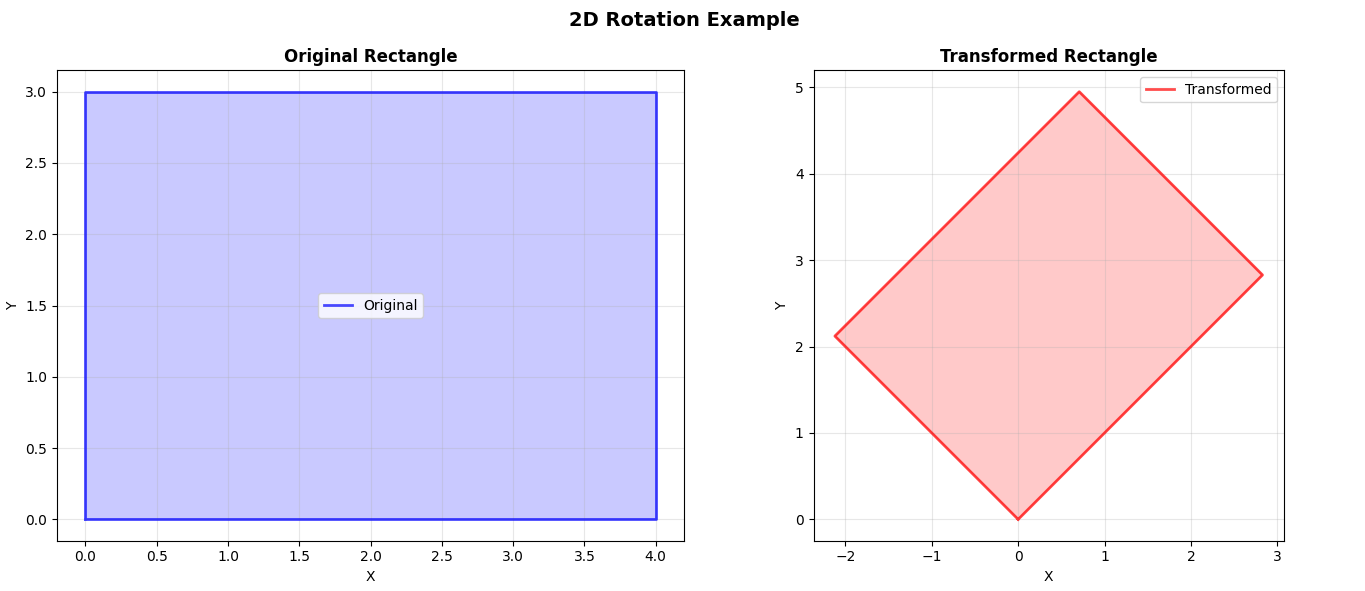
\includegraphics[width=0.8\textwidth]{fig/Screenshot 2026-02-09 154121.png}
    \caption{2D Rotation: Original shape (left) vs Rotated shape by 90° (right)}
\end{figure}

\newpage
%===========================================
% TASK 3: 2D SCALING
%===========================================
\section{2D Scaling}

\subsection{Title of Lab Activity}
Implementation of 2D Scaling transformation using homogeneous coordinates to resize objects by specified scaling factors in x and y directions.

\subsection{Algorithm used for drawing line}
Digital Differential Analyzer (DDA) and Bresenham's algorithm are fundamental line rasterization techniques. For this lab, Matplotlib handles the rendering pipeline for clear visualization.

\textbf{Scaling Algorithm Steps:}
\begin{enumerate}
    \item Input scaling factors: $s_x$ (horizontal) and $s_y$ (vertical)
    \item Construct the scaling matrix:
    $$S = \begin{bmatrix} s_x & 0 & 0 \\ 0 & s_y & 0 \\ 0 & 0 & 1 \end{bmatrix}$$
    \item Convert 2D points to homogeneous coordinates
    \item Apply transformation: $P' = S \times P$
    \item Extract scaled coordinates from result
    \item Note: Scaling is performed about the origin (0,0)
\end{enumerate}

\subsection{Source Code}
\begin{lstlisting}[language=Python, caption=2D Scaling Implementation]
@staticmethod
def scaling_matrix(sx, sy):
    """
    Create a scaling transformation matrix.
    
    Args:
        sx: Scaling factor in x-axis
        sy: Scaling factor in y-axis
        
    Returns:
        3x3 scaling matrix
    """
    return np.array([
        [sx, 0, 0],
        [0, sy, 0],
        [0, 0, 1]
    ], dtype=float)

# Example usage
tri = Shape2D([(0, 0), (4, 0), (2, 4)], name="Triangle")
scale = Transformation2D.scaling_matrix(2, 1.5)
tri.apply_transformation(scale)
Visualizer2D.plot_comparison(original_tri, tri, title="2D Scaling")
\end{lstlisting}

\subsection{Output}
\begin{figure}[H]
    \centering
    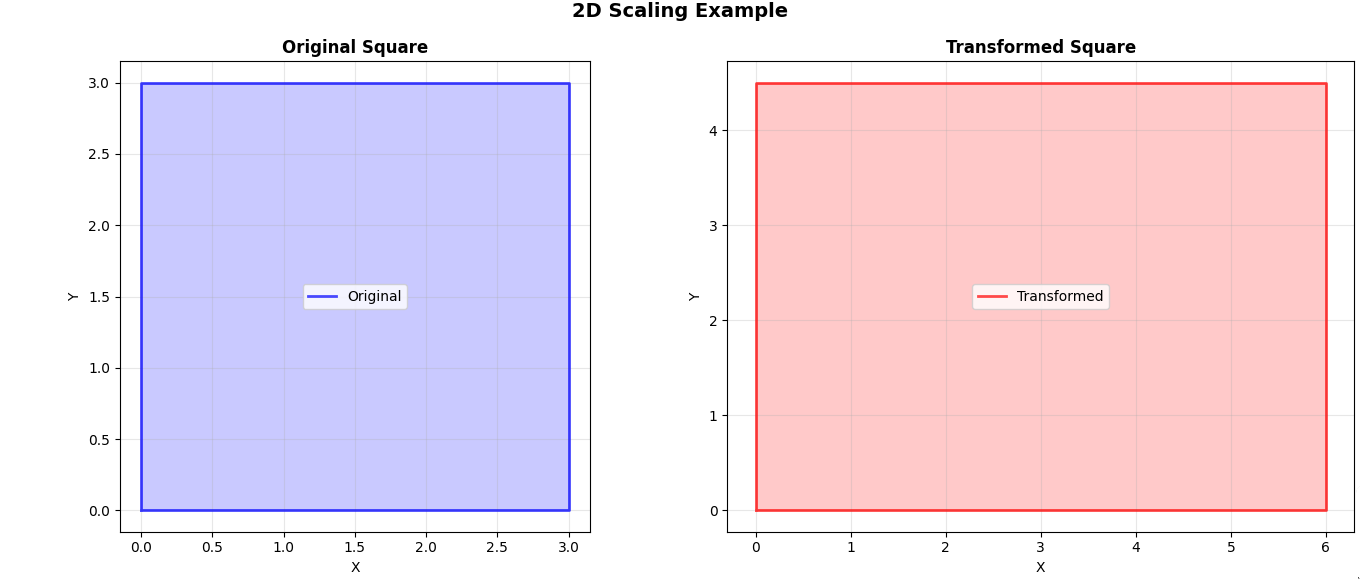
\includegraphics[width=0.8\textwidth]{fig/Screenshot 2026-02-09 154142.png}
    \caption{2D Scaling: Original shape (left) vs Scaled shape (2x, 1.5x) (right)}
\end{figure}

\newpage
%===========================================
% TASK 4: 2D REFLECTION
%===========================================
\section{2D Reflection}

\subsection{Title of Lab Activity}
Implementation of 2D Reflection transformation using homogeneous coordinates to create mirror images of objects about different axes.

\subsection{Algorithm used for drawing line}
Digital Differential Analyzer (DDA) and Bresenham's line algorithm are fundamental for line rasterization. The reflection transformation uses matrix operations while Matplotlib provides the visualization framework.

\textbf{Reflection Algorithm Steps:}
\begin{enumerate}
    \item Choose the reflection axis: X-axis, Y-axis, or Origin
    \item Construct the appropriate reflection matrix:
    \begin{itemize}
        \item X-axis: $R_x = \begin{bmatrix} 1 & 0 & 0 \\ 0 & -1 & 0 \\ 0 & 0 & 1 \end{bmatrix}$
        \item Y-axis: $R_y = \begin{bmatrix} -1 & 0 & 0 \\ 0 & 1 & 0 \\ 0 & 0 & 1 \end{bmatrix}$
        \item Origin: $R_o = \begin{bmatrix} -1 & 0 & 0 \\ 0 & -1 & 0 \\ 0 & 0 & 1 \end{bmatrix}$
    \end{itemize}
    \item Convert 2D points to homogeneous coordinates
    \item Apply transformation: $P' = R \times P$
    \item Extract reflected coordinates from result
\end{enumerate}

\subsection{Source Code}
\begin{lstlisting}[language=Python, caption=2D Reflection Implementation]
@staticmethod
def reflection_matrix(axis='x'):
    """
    Create a reflection transformation matrix.
    
    Args:
        axis: 'x' for reflection about x-axis, 'y' for y-axis, 'origin' for origin
        
    Returns:
        3x3 reflection matrix
    """
    if axis == 'x':
        # Reflection about x-axis
        return np.array([
            [1, 0, 0],
            [0, -1, 0],
            [0, 0, 1]
        ], dtype=float)
    elif axis == 'y':
        # Reflection about y-axis
        return np.array([
            [-1, 0, 0],
            [0, 1, 0],
            [0, 0, 1]
        ], dtype=float)
    elif axis == 'origin':
        # Reflection about origin
        return np.array([
            [-1, 0, 0],
            [0, -1, 0],
            [0, 0, 1]
        ], dtype=float)

# Example usage
tri = Shape2D([(0, 0), (3, 0), (1.5, 2)], name="Triangle")
ref = Transformation2D.reflection_matrix('y')
tri.apply_transformation(ref)
Visualizer2D.plot_comparison(original_tri, tri, title="2D Reflection")
\end{lstlisting}

\subsection{Output}
\begin{figure}[H]
    \centering
    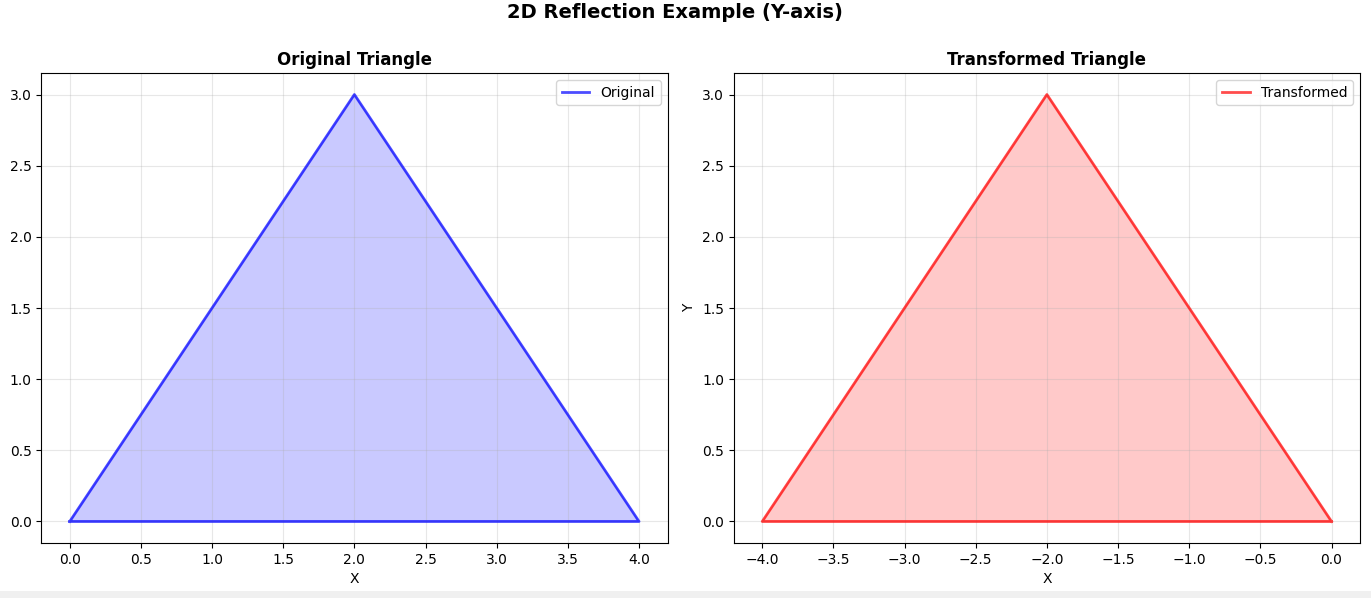
\includegraphics[width=0.8\textwidth]{fig/Screenshot 2026-02-09 154159.png}
    \caption{2D Reflection: Original shape (left) vs Reflected shape about Y-axis (right)}
\end{figure}

\newpage
%===========================================
% TASK 5: 2D SHEARING
%===========================================
\section{2D Shearing}

\subsection{Title of Lab Activity}
Implementation of 2D Shearing transformation using homogeneous coordinates to distort objects by shifting points proportionally along one axis.

\subsection{Algorithm used for drawing line}
Digital Differential Analyzer (DDA) and Bresenham's line algorithm provide the foundation for line rendering. Shearing transformation modifies coordinate relationships using matrix operations.

\textbf{Shearing Algorithm Steps:}
\begin{enumerate}
    \item Input shearing parameters: $sh_x$ (shear in x-direction) and $sh_y$ (shear in y-direction)
    \item Construct the shearing matrix:
    $$Sh = \begin{bmatrix} 1 & sh_x & 0 \\ sh_y & 1 & 0 \\ 0 & 0 & 1 \end{bmatrix}$$
    \item Convert 2D points to homogeneous coordinates
    \item Apply transformation: $P' = Sh \times P$
    \item Extract sheared coordinates from result
    \item Note: $sh_x$ shifts points horizontally based on y-coordinate, $sh_y$ shifts vertically based on x-coordinate
\end{enumerate}

\subsection{Source Code}
\begin{lstlisting}[language=Python, caption=2D Shearing Implementation]
@staticmethod
def shearing_matrix(shx=0, shy=0):
    """
    Create a shearing transformation matrix.
    
    Args:
        shx: Shearing factor in x-direction
        shy: Shearing factor in y-direction
        
    Returns:
        3x3 shearing matrix
    """
    return np.array([
        [1, shx, 0],
        [shy, 1, 0],
        [0, 0, 1]
    ], dtype=float)

# Example usage
square = Shape2D([(0, 0), (2, 0), (2, 2), (0, 2)], name="Square")
shear = Transformation2D.shearing_matrix(shx=0.5, shy=0)
square.apply_transformation(shear)
Visualizer2D.plot_comparison(original_square, square, title="2D Shearing")
\end{lstlisting}

\subsection{Output}
\begin{figure}[H]
    \centering
    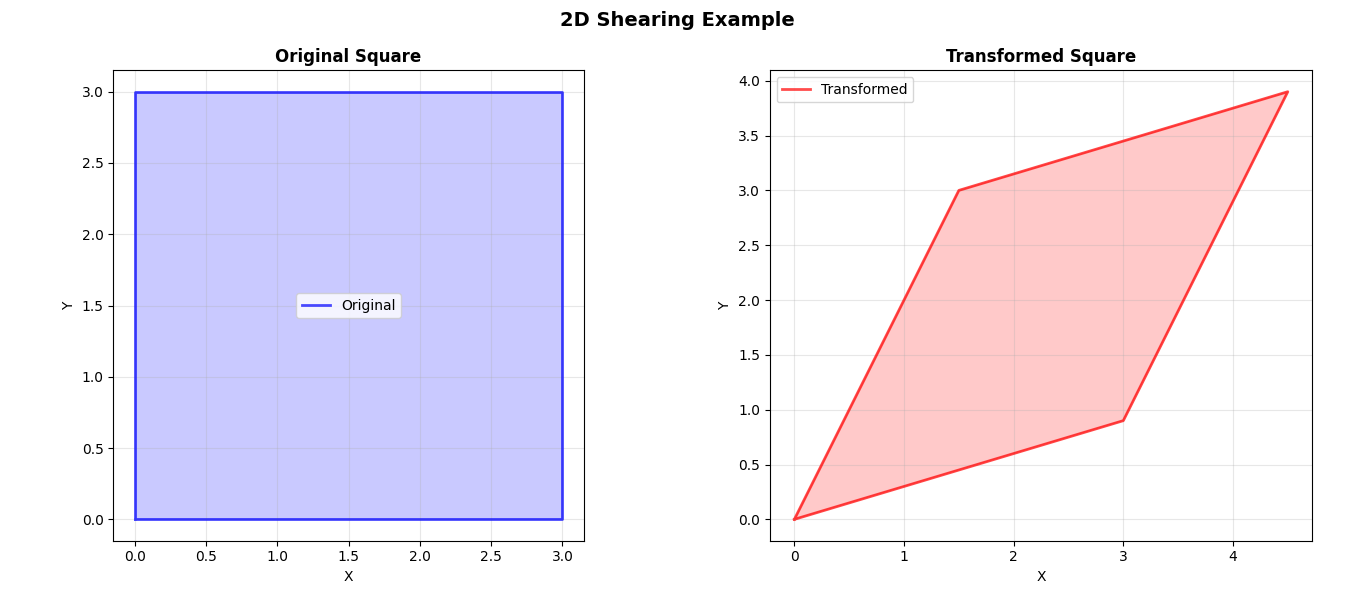
\includegraphics[width=0.8\textwidth]{fig/Screenshot 2026-02-09 154209.png}
    \caption{2D Shearing: Original shape (left) vs Sheared shape (shx=0.5) (right)}
\end{figure}

\newpage
%===========================================
% TASK 6: COMPOSITE TRANSFORMATIONS
%===========================================
\section{Composite Transformations}

\subsection{Title of Lab Activity}
Implementation of Composite Transformations using homogeneous coordinates to combine multiple transformation operations (Translation, Rotation, Scaling, Reflection, and Shearing) into a single matrix operation.

\subsection{Algorithm used for drawing line}
Digital Differential Analyzer (DDA) and Bresenham's line algorithm handle the underlying line rasterization. Composite transformations leverage matrix multiplication properties for efficient multi-step transformations.

\textbf{Composite Transformation Algorithm Steps:}
\begin{enumerate}
    \item Define individual transformation matrices: $T$ (Translation), $R$ (Rotation), $S$ (Scaling), $Ref$ (Reflection), $Sh$ (Shearing)
    \item Determine the order of transformations (matrix multiplication is not commutative)
    \item Compute composite matrix: $C = T_n \times T_{n-1} \times \ldots \times T_2 \times T_1$
    \item Apply composite transformation: $P' = C \times P$
    \item Example: Translation → Rotation → Scaling → Shearing
    $$C = Sh \times S \times R \times T$$
\end{enumerate}

\subsection{Source Code}
\begin{lstlisting}[language=Python, caption=Composite Transformations Implementation]
@staticmethod
def composite_transformation(*matrices):
    """
    Combine multiple transformation matrices into a single composite matrix.
    Matrices are applied left to right (first matrix is applied first).
    
    Args:
        *matrices: Variable number of 3x3 transformation matrices
        
    Returns:
        3x3 composite transformation matrix
    """
    result = np.eye(3)
    for matrix in matrices:
        result = matrix @ result
    return result

# Example: 4+ Transformations Combined
rect = Shape2D([(0, 0), (2, 0), (2, 1), (0, 1)], name="Rectangle")

# Individual transformations
trans_matrix = Transformation2D.translation_matrix(2, 1)
rot_matrix = Transformation2D.rotation_matrix(45)
scale_matrix = Transformation2D.scaling_matrix(1.5, 1.5)
shear_matrix = Transformation2D.shearing_matrix(0.3, 0)
ref_matrix = Transformation2D.reflection_matrix('y')

# Combine 5 transformations: T→R→S→Sh→Ref
composite = Transformation2D.composite_transformation(
    ref_matrix, shear_matrix, scale_matrix, rot_matrix, trans_matrix
)

rect.apply_transformation(composite)
Visualizer2D.plot_comparison(original_rect, rect, title="Composite Transformations")
\end{lstlisting}

\subsection{Output}
\begin{figure}[H]
    \centering
    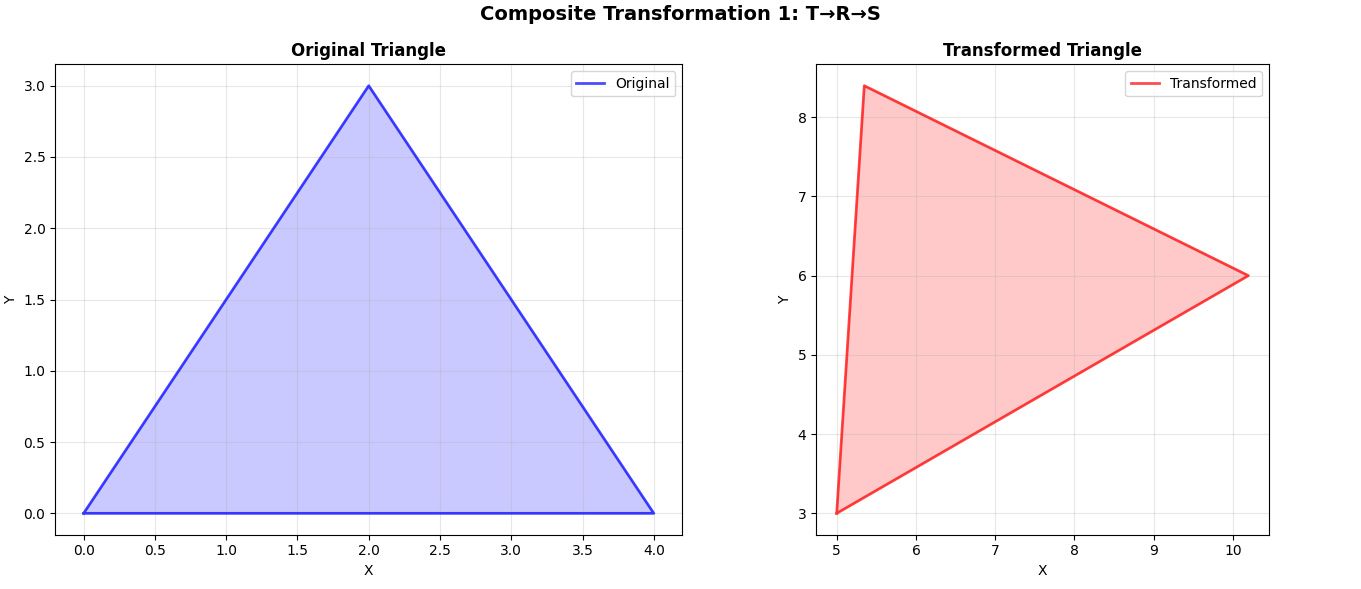
\includegraphics[width=0.8\textwidth]{fig/Screenshot 2026-02-09 154221.png}
    \caption{Composite Transformations: Original shape (left) vs Shape after 5 combined transformations (right)}
\end{figure}

\newpage
%===========================================
% CONCLUSION
%===========================================
\section{Conclusion}

This laboratory exercise provided comprehensive hands-on experience with fundamental 2D transformation techniques in computer graphics. The six core transformations implemented demonstrate the power and elegance of homogeneous coordinate systems for unified geometric operations.

\textbf{Key Learnings:}
\begin{itemize}
    \item \textbf{Homogeneous Coordinates:} The use of 3×3 matrices for 2D transformations enables uniform representation and easy composition of multiple transformations
    \item \textbf{Matrix Multiplication:} All transformations are performed through matrix multiplication, making the operations mathematically consistent and computationally efficient
    \item \textbf{Translation:} Moving objects by adding constant values to coordinates, implemented as matrix multiplication using homogeneous coordinates
    \item \textbf{Rotation:} Rotating objects about the origin using trigonometric functions, maintaining shape and size while changing orientation
    \item \textbf{Scaling:} Resizing objects by multiplying coordinates with scaling factors, allowing independent control over x and y dimensions
    \item \textbf{Reflection:} Creating mirror images of objects about specified axes (x-axis, y-axis, or origin) using sign inversion
    \item \textbf{Shearing:} Distorting objects by proportionally shifting coordinates, useful for creating slanted or skewed effects
    \item \textbf{Composite Transformations:} Combining multiple transformations into single operations, demonstrating matrix multiplication's non-commutative property
\end{itemize}

\textbf{Technical Insights:}
\begin{itemize}
    \item Understanding the mathematical foundation of computer graphics transformations
    \item The importance of homogeneous coordinates in unifying different transformation types
    \item How matrix representations enable efficient computer implementation of geometric operations
    \item The relationship between mathematical theory and practical graphics programming
    \item Matrix multiplication order significance in composite transformations
    \item The computational efficiency gained by combining multiple operations into single matrix multiplication
\end{itemize}

\textbf{Observations:}
\begin{itemize}
    \item All basic transformations preserve certain geometric properties (angles in rotation, ratios in scaling)
    \item Homogeneous coordinate system allows seamless combination of transformations
    \item The matrix approach scales efficiently for complex graphics applications
    \item Composite transformations demonstrate the power of matrix mathematics in graphics
    \item Reflection and shearing add creative possibilities for object manipulation
    \item These fundamental transformations form the building blocks for advanced graphics operations including 3D transformations
\end{itemize}

The laboratory exercise successfully demonstrated how mathematical concepts translate into practical computer graphics implementations. The complete set of six transformations provides essential knowledge for advanced graphics programming, animation systems, and 3D transformation pipelines. Understanding these fundamentals is crucial for developing sophisticated graphics applications and game engines.

\end{document}